Report cards are typically compiled and communicated annually.  However, the time window that
constitutes a year differs from report card to report card.  Many environmental report cards
communicate on data collected within a financial year.  This schedule provides a reporting window
that is consistent with other management and governmental considerations.  Others use a time window
that naturally aligns with the cycle of some major underlying environmental gradient - such as
wet/dry season. For this project, we are adopting using the same water year (1st Oct -- 31 Sept)
definition as the AIMS inshore Water Quality Marine Monitoring Program \citep{Lonborg-MMP-2015}.

The Great Barrier Reef Marine Park (GBR)spans nearly 14$^\circ$ of latitude and covers approximately
344,400km$^2$.

- spanning multiple jurisdictions/pressures as well as distance offshore - more useful to partition
the GBR into smaller more homogeneous zones representing combinations of region and water body.  -
Six regions (Cape York, Wet Tropics, Dry Tropics, Mackay Whitsunday, Fitzroy and Burnett Mary) -
Four water bodies (Enclosed Coastal, Open Coastal, Midshelf and Offshore) - define each...
 
  \arrayrulecolor[rgb]{0.06,0.25,0.49}
 \LTcapwidth=\linewidth
 \setlength\aboverulesep{0pt}\setlength\belowrulesep{0pt}
 \setlength\cmidrulekern{1pt}\setlength\cmidrulewidth{1pt}
 \renewcommand\arraystretch{1.2}\setlength\tabcolsep{5pt}
 %\begin{landscape}
 \begin{table}[h]\caption{Great Barrier Reef spatial Zones and associated Regions and Water bodies.}\label{tab:spatial}
 %\begin{center}
 \scriptsize
 \begin{tabular}{
 !{\color[rgb]{0.06,0.25,0.49}\VRule[1pt]} p{25em}
 !{\color[rgb]{0.06,0.25,0.49}\vline} l
 !{\color[rgb]{0.06,0.25,0.49}\vline} l
 !{\color[rgb]{0.06,0.25,0.49}\vline} l
 !{\color[rgb]{0.06,0.25,0.49}\VRule[1pt]}
 }
 \arrayrulecolor[rgb]{0.06,0.25,0.49}\specialrule{1pt}{0pt}{0pt} %top border
 \rowcolor[rgb]{0.53,0.62,0.74} 
 %\multicolumn{1}{!{\color[rgb]{0.06,0.25,0.49}\VRule[1pt]}l}}{\whiteHeader{{GBRMPA Zone}}} & 
 \multicolumn{1}{l}{\whiteHeader{{GBRMPA Zone}}} & 
 \multicolumn{1}{l}{\whiteHeader{{Zone}}} & 
 \multicolumn{1}{l}{\whiteHeader{{Region}}} & 
 \whiteHeader{{Water body}}\\ 
 \cmidrule{1-4} 
Enclosed\_Coastal\_Cape\_York & Enclosed\_Coastal\_Cape York & Cape York & Enclosed Coastal \\ 
  Enclosed\_Coastal\_Terrain\_NRM & Enclosed\_Coastal\_Wet Tropics & Wet Tropics & Enclosed Coastal \\ 
  Enclosed\_Coastal\_Burdekin\_Dry\_Tropics\_NRM & Enclosed\_Coastal\_Dry Tropics & Dry Tropics & Enclosed Coastal \\ 
  Enclosed\_Coastal\_Mackay\_Whitsunday\_NRM\_Group & Enclosed\_Coastal\_Mackay Whitsunday & Mackay Whitsunday & Enclosed Coastal \\ 
  Enclosed\_Coastal\_Fitzroy\_Basin\_Association & Enclosed\_Coastal\_Fitzroy & Fitzroy & Enclosed Coastal \\ 
  Enclosed\_Coastal\_Burnett\_Mary\_Regional\_Group\_for\_NRM & Enclosed\_Coastal\_Burnett Mary & Burnett Mary & Enclosed Coastal \\ 
   \cline{1-4}Open\_Coastal\_Cape\_York & Open\_Coastal\_Cape York & Cape York & Open Coastal \\ 
  Open\_Coastal\_Terrain\_NRM & Open\_Coastal\_Wet Tropics & Wet Tropics & Open Coastal \\ 
  Open\_Coastal\_Burdekin\_Dry\_Tropics\_NRM & Open\_Coastal\_Dry Tropics & Dry Tropics & Open Coastal \\ 
  Open\_Coastal\_Mackay\_Whitsunday\_NRM\_Group & Open\_Coastal\_Mackay Whitsunday & Mackay Whitsunday & Open Coastal \\ 
  Open\_Coastal\_Fitzroy\_Basin\_Association & Open\_Coastal\_Fitzroy & Fitzroy & Open Coastal \\ 
  Open\_Coastal\_Burnett\_Mary\_Regional\_Group\_for\_NRM & Open\_Coastal\_Burnett Mary & Burnett Mary & Open Coastal \\ 
   \cline{1-4}Midshelf\_Cape\_York & Midshelf\_Cape York & Cape York & Midshelf \\ 
  Midshelf\_Terrain\_NRM & Midshelf\_Wet Tropics & Wet Tropics & Midshelf \\ 
  Midshelf\_Burdekin\_Dry\_Tropics\_NRM & Midshelf\_Dry Tropics & Dry Tropics & Midshelf \\ 
  Midshelf\_Mackay\_Whitsunday\_NRM\_Group & Midshelf\_Mackay Whitsunday & Mackay Whitsunday & Midshelf \\ 
  Midshelf\_Fitzroy\_Basin\_Association & Midshelf\_Fitzroy & Fitzroy & Midshelf \\ 
  Midshelf\_Burnett\_Mary\_Regional\_Group\_for\_NRM & Midshelf\_Burnett Mary & Burnett Mary & Midshelf \\ 
   \cline{1-4}Offshore\_Cape\_York & Offshore\_Cape York & Cape York & Offshore \\ 
  Offshore\_Terrain\_NRM & Offshore\_Wet Tropics & Wet Tropics & Offshore \\ 
  Offshore\_Burdekin\_Dry\_Tropics\_NRM & Offshore\_Dry Tropics & Dry Tropics & Offshore \\ 
  Offshore\_Mackay\_Whitsunday\_NRM\_Group & Offshore\_Mackay Whitsunday & Mackay Whitsunday & Offshore \\ 
  Offshore\_Fitzroy\_Basin\_Association & Offshore\_Fitzroy & Fitzroy & Offshore \\ 
  Offshore\_Burnett\_Mary\_Regional\_Group\_for\_NRM & Offshore\_Burnett Mary & Burnett Mary & Offshore \\ 
   \bottomrule
 \end{tabular}
 %\end{center}
 \end{table} %\end{landscape}


  

\begin{figure}[ptbh] \includegraphics[width=1\linewidth]{figures/Maps/Map_region_waterbody\res.pdf}
\caption{Great Barrier Reef Zones (Regions and Water Bodies).}\label{fig:Map_region_waterbody}
\end{figure}
   
  \arrayrulecolor[rgb]{0.06,0.25,0.49}
 \LTcapwidth=\linewidth
 \setlength\aboverulesep{0pt}\setlength\belowrulesep{0pt}
 \setlength\cmidrulekern{1pt}\setlength\cmidrulewidth{1pt}
 \renewcommand\arraystretch{1.2}\setlength\tabcolsep{5pt}
 \begin{table}[h]\caption{Summary of used data sources.}\label{tab:sources}
 %\begin{center}
 \scriptsize
 \begin{tabular}{
 !{\color[rgb]{0.06,0.25,0.49}\VRule[1pt]} p{6em}
 !{\color[rgb]{0.06,0.25,0.49}\vline} l
 !{\color[rgb]{0.06,0.25,0.49}\vline} l
 !{\color[rgb]{0.06,0.25,0.49}\VRule[1pt]}
 }
 \arrayrulecolor[rgb]{0.06,0.25,0.49}\specialrule{1pt}{0pt}{0pt} %top border
 \rowcolor[rgb]{0.53,0.62,0.74} 
 \multicolumn{1}{!{\color[rgb]{0.06,0.25,0.49}\VRule[1pt]}l}{\whiteHeader{{Source}}} & 
 \multicolumn{1}{l}{\whiteHeader{{Custodian}}} & 
 \whiteHeader{{Description}}\\ 
 \cmidrule{1-3} 
AIMS Insitu & AIMS & AIMS inshore monitoring program Niskin data \\ 
   \cline{1-3}AIMS FLNTU & AIMS & AIMS inshore monitoring program FLNTU logger data \\ 
   \cline{1-3}Satellite & BOM & BOM: Catalog http://ereeftds.bom.gov.au/ereefs/tds/catalog/ereef/mwq/P1D/2002/catalog.html \\ 
   \cline{1-3}eReefs & eReefs & \textcolor{red}{provide a description in ../parameters/sources.csv} \\ 
   \cline{1-3}eReefs926 & eReefs & eReefs: http://dapds00.nci.org.au/thredds/catalog/fx3/gbr4\_bgc\_926/catalog.html \\ 
   \bottomrule
 \end{tabular}
 %\end{center}
 \end{table}



\subsection{Indicators}

One of the biggest challenges of report card development is the selection of appropriate indicators
from amongst a potentially very large candidate pool.  Since the outcomes, conclusions and
implications are all dependent on the indicators selected, the selection process is one of the most
influential steps and has justifiably received a great deal of attention.

As part of their ecosystem report card framework, \citet{Harwell-1999} urged that the alignment of
scientific information with societal goals and objectives should be the guiding principal of
indicator selection.  In their framework, clearly articulated societal goals and objectives (a
combination of societal values and scientific knowledge, such as restored and sustainable wetland
system) are translated into Essential Ecosystem Characteristics (EECs) that represent a set of
generic attributes that further refine the broad goals (such as water quality, sediment quality,
habitat quality, ecological processes).  The EEC's are then further translated into a set of
scientific informed indicators that are measured or monitored to indicate the status of trends or
states associated with the EEC's.
  
There have since been numerous studies that have focused on providing more formal, objective
criterion for indicator selection \citep{Dauvin-2008, Emerson-2012, Flint-2012, James-2012}.  Whilst
the specifics vary, most can be broadly encapsulated by a \citet{Dauvin-2008}'s contextual
implementation of the \citet{Doran-1981}'s SMART (Simple, Measurable, Achievable, Realistic, and
Time limited) principle.  A 'good' indicator should be representative, easily interpreted, broadly
comparable, sensitive to change and have a reference or guideline value.  To be `useful', an
indicator must be approved by international consensus, be well grounded and documented, have a
reasonable cost/benefit ratio and have adequate historical and on-going spatial-temporal coverage.
\citet{Flint-2012} and \citet{James-2012} further developed numerical scoring systems to help
evaluate indicators objectively.  Nevertheless, \citep{Neary-2012} warned against the potential to
manipulate an index by saturating with inappropriate or biased indicators and whilst recommending
that an index comprise of at least seven indicators, they did advocate that the type of indicator is
more important than the number of indicators._

Since final outcomes are likely to be highly influenced by indicator choice, the robustness and
sensitivity of both indicators and final outcomes to changes in ecosystem health should be
understood if not formally investigated as part of the indicator selection process
\citep{Dobbie-2013}.  Sensitivity analyses can involve:

\begin{itemize}
\item simulating changes in the underlying data of different magnitudes and estimating the resulting
sensitivity (percentage or probability of change) expressed by the indicator
\item estimating the effect of past perturbations on the indicator hindcasted from on historical
data
\end{itemize}

As stressed above, indicators should align intimately with report card objectives.  Yet in the more
broad ecosystem report card frameworks, such indicators are often too general to be measurable.
Therefore, in such cases, the indicators are further sub-divided into progressively more specific
measures.  For example, an indicator of water quality might comprise sub-indicators of nutrients,
metals and physico-chemistry which in turn might be represented by more specific measures such as
total nitrogen, mercury, dissolved oxygen, pH etc.

The resulting design is a hierarchical structure in which sub-indicators (etc) are nested within
indicators and spatial scales are nested from entire regions, sub-regions or zones down to
individual sites or sampling units.  One of the strengths of such a hierarchical report card
framework is that the inherent inbuilt redundancy allows for the addition, deletion or exchange of
finer scale items (sites and actual measured variables) with minimum disruption to the actual report
indicators.  That is, the indicator is relatively robust to some degree of internal makeup.
Furthermore, by abstracting away the fine details of an indicator, similar indicators from different
report cards (each potentially comprising different sampling designs) are more directly comparably.
For example, in different report cards that include water quality, a water quality indicator of
'water clarity' might comprise different Measures (e.g. suspended solids, NTU, Secchi depth etc)
collected from different sources (e.g. satellite, in situ loggers or hand samples), yet provided
each of these water clarity indicators are well calibrated, it should be possible to compare state
and trend across the report cards.
  
  \arrayrulecolor[rgb]{0.06,0.25,0.49}
 \LTcapwidth=\linewidth
 \setlength\aboverulesep{0pt}\setlength\belowrulesep{0pt}
 \setlength\cmidrulekern{1pt}\setlength\cmidrulewidth{1pt}
 \renewcommand\arraystretch{1.2}\setlength\tabcolsep{5pt}
 \begin{table}[h]\caption{Water Quality Measure hierarchy specifying which Measures contribute to which Subindicators and which Subindicators contribute to which Indicators.}\label{tab:measures}
 \begin{center}
 \scriptsize
 \begin{tabular}{
 !{\color[rgb]{0.06,0.25,0.49}\VRule[1pt]} p{6em}
 !{\color[rgb]{0.06,0.25,0.49}\vline} l
 !{\color[rgb]{0.06,0.25,0.49}\vline} l
 !{\color[rgb]{0.06,0.25,0.49}\vline} l
 !{\color[rgb]{0.06,0.25,0.49}\vline} l
 !{\color[rgb]{0.06,0.25,0.49}\VRule[1pt]}
 }
 \arrayrulecolor[rgb]{0.06,0.25,0.49}\specialrule{1pt}{0pt}{0pt} %top border
 \rowcolor[rgb]{0.53,0.62,0.74} 
 \multicolumn{1}{!{\color[rgb]{0.06,0.25,0.49}\VRule[1pt]} p{6em}}{\whiteHeader{{Indicator}}} & 
 \multicolumn{1}{l}{\whiteHeader{{Subindicator}}} & 
 \multicolumn{1}{l}{\whiteHeader{{Measure}}} & 
 \multicolumn{1}{l}{\whiteHeader{{Label}}} & 
 \whiteHeader{{Units}}\\ 
 \cmidrule{1-5} 
 \cline{1-5}Water Quality & Productivity & chl & Chlorophyll & µgL^{-1} \\ 
   \cline{3-5} \cline{2-5}Water Quality & Water Clarity & nap & TSS & mgL^{-1} \\ 
   \cline{3-5}Water Quality & Water Clarity & ntu & NTU & NTU \\ 
   \cline{3-5}Water Quality & Water Clarity & sd & Secchi & m \\ 
   \cline{3-5} \cline{2-5}Water Quality & Nutrients & NOx & NOx & µgL^{-1} \\ 
   \bottomrule
 \end{tabular}
 \end{center}
 \end{table}
   
   
  
\subsection{AIMS insitu samples}

The AIMS component of MMP inshore water quality monitoring sampling program has been designed to
quantify spatial and temporal patterns in inshore water quality, particularly in the context of
catchment loads.  Details of the sampling design are outlined in \citep{Lonborg-MMP-2015}.  From
2006--2014, AIMS visited 20 sites, three times per year (roughly corresponding to wet, early and
late dry seasons), see Figures~\ref{fig:AIMS_insitu_map} and \ref{fig:AIMS_insitu_spatial_temporal}.
The sites were largely selected along approximate north-south transects proximal to major rivers so
as to provide samples along an expected water quality gradients (exposure to runoff).  Following a
review in 2014, the design was modified to intensify the spatial (32 sites) and temporal (typically
between 5 and 10 samples per year) coverage of the sampling program.  In particular, additional
sampling effort was applied around three priority focal areas (Russell-Mulgrave, Tully and
Burdekin).

\begin{figure}[ptbh]
\includegraphics[width=1\linewidth]{{figures/Maps/Insitu_sites/Map_insitu1\res}.pdf}
\caption{Map of AIMS in situ samples.}\label{fig:AIMS_insitu_map}
\end{figure}

\begin{figure}[ptbh]
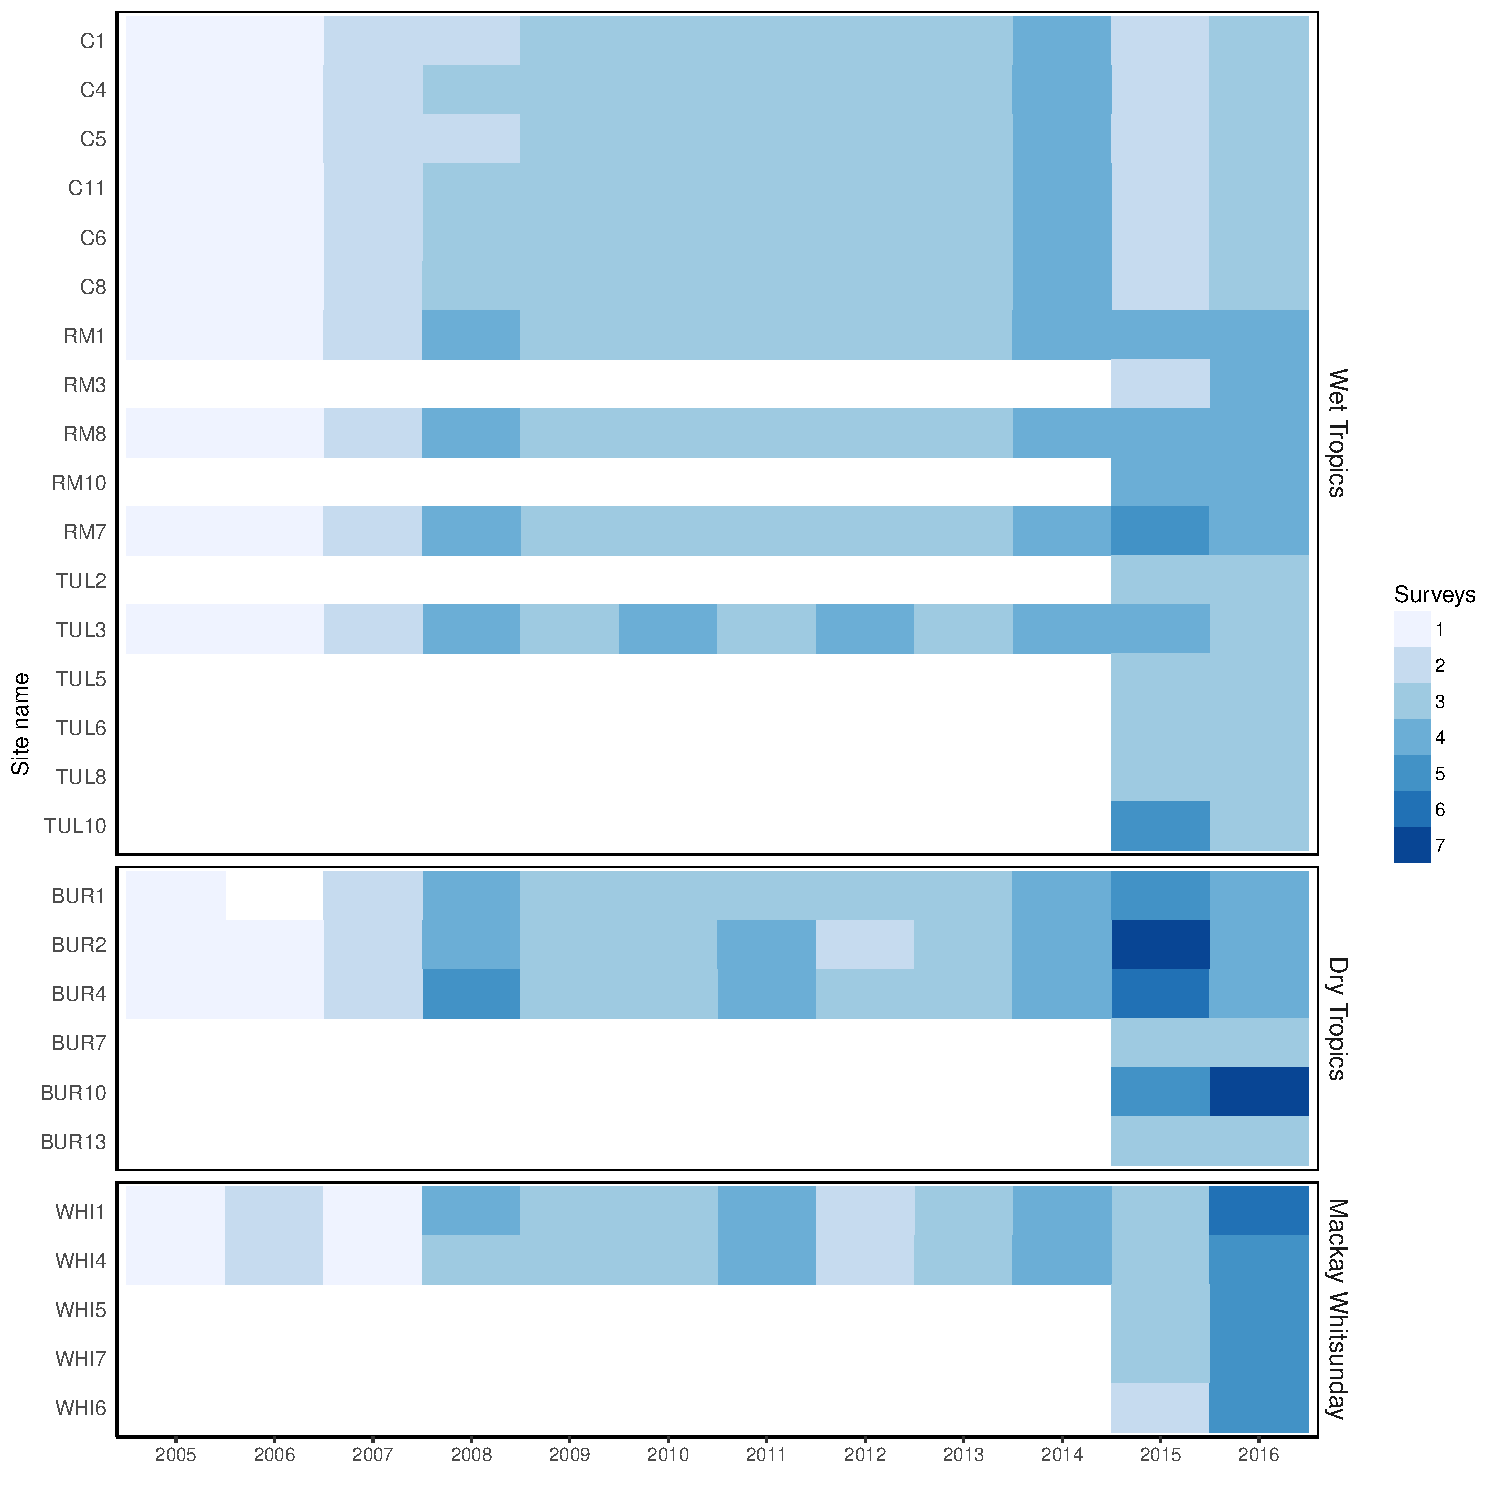
\includegraphics[width=1\linewidth]{figures/Maps/Insitu_sites/Samples_spatial_temporal.pdf}
\caption{Spatial and temporal distribution of AIMS insitu samples.  Sites names follow Great Barrier
Reef Marine Park Authority (GBRMPA) and sites are arranged north to south into the focal
Regions. Blue shading of tiles denotes the number of surveys conducted in the year at each
site.}\label{fig:AIMS_insitu_spatial_temporal}
\end{figure}
 
  \arrayrulecolor[rgb]{0.06,0.25,0.49}
 \LTcapwidth=\linewidth
 \setlength\aboverulesep{0pt}\setlength\belowrulesep{0pt}
 \setlength\cmidrulekern{1pt}\setlength\cmidrulewidth{1pt}
 \renewcommand\arraystretch{1.2}\setlength\tabcolsep{5pt}
 \begin{table}\caption{Measures collected in AIMS MMP insitu inshore water quality monitoring program.  NOx is the sum of NO$_2$ and NO$_3$.  Data used are annual means of depth weighted averages per site.}\label{tab:insitu.measures}
 %\begin{center}
 \scriptsize
 \begin{tabular}{
 !{\color[rgb]{0.06,0.25,0.49}\VRule[1pt]} p{10em}
 !{\color[rgb]{0.06,0.25,0.49}\vline} l
 !{\color[rgb]{0.06,0.25,0.49}\vline} p{15em}
 !{\color[rgb]{0.06,0.25,0.49}\vline} l
 !{\color[rgb]{0.06,0.25,0.49}\vline} l
 !{\color[rgb]{0.06,0.25,0.49}\vline} l
 !{\color[rgb]{0.06,0.25,0.49}\VRule[1pt]}
 }
 \arrayrulecolor[rgb]{0.06,0.25,0.49}\specialrule{1pt}{0pt}{0pt} %top border
 \rowcolor[rgb]{0.53,0.62,0.74} 
 \multicolumn{1}{!{\color[rgb]{0.06,0.25,0.49}\VRule[1pt]}l}{\whiteHeader{{Measure}}} & 
 \multicolumn{1}{l}{\whiteHeader{{Variable}}} & 
 \multicolumn{1}{l}{\whiteHeader{{Description}}} & 
 \multicolumn{1}{l}{\whiteHeader{{Abbreviation}}} & 
 \multicolumn{1}{l}{\whiteHeader{{Conversion}}} & 
 \whiteHeader{{Units}}\\ 
 \cmidrule{1-6} 
Chlorophyll-a & DRIFTCHL\_UGPERL.wm & Chlorophyll-a (µg/L) & chl & x1 & µgL^{-1} \\ 
   \cline{1-6}Total Suspended Solids & TSS\_MGPERL.wm & Suspended solids (mg/L) & nap & x1 & mgL^{-1} \\ 
   \cline{1-6}Secchi Depth & SECCHI\_DEPTH.wm & Secchi depth (m) & sd & x1 & m \\ 
   \cline{1-6}NOx & NOX.wm & Nitrite and Nitrate measured by microanalyser (µM/L) & NOx & x14 & µgL^{-1} \\ 
   \bottomrule
 \end{tabular}
 %\end{center}
 \end{table}


\clearpage

\subsection{AIMS FLNTU samples}
  
Combination continuous Flourometer and Turbidity Sensors (hereafter FLNTU) loggers were deployed at
15 of the AIMS MMP inshore water quality monitoring sites.
 
  \arrayrulecolor[rgb]{0.06,0.25,0.49}
 \LTcapwidth=\linewidth
 \setlength\aboverulesep{0pt}\setlength\belowrulesep{0pt}
 \setlength\cmidrulekern{1pt}\setlength\cmidrulewidth{1pt}
 \renewcommand\arraystretch{1.2}\setlength\tabcolsep{5pt}
 \begin{table}[h]\caption{Measures collected in AIMS MMP flntu inshore water quality monitoring program. Data used are daily means per site.}\label{tab:flntu.measures}
 %\begin{center}
 \scriptsize
 \begin{tabular}{
 !{\color[rgb]{0.06,0.25,0.49}\VRule[1pt]} p{10em}
 !{\color[rgb]{0.06,0.25,0.49}\vline} l
 !{\color[rgb]{0.06,0.25,0.49}\vline} p{15em}
 !{\color[rgb]{0.06,0.25,0.49}\vline} l
 !{\color[rgb]{0.06,0.25,0.49}\vline} l
 !{\color[rgb]{0.06,0.25,0.49}\vline} l
 !{\color[rgb]{0.06,0.25,0.49}\VRule[1pt]}
 }
 \arrayrulecolor[rgb]{0.06,0.25,0.49}\specialrule{1pt}{0pt}{0pt} %top border
 \rowcolor[rgb]{0.53,0.62,0.74} 
 \multicolumn{1}{!{\color[rgb]{0.06,0.25,0.49}\VRule[1pt]}l}{\whiteHeader{{Measure}}} & 
 \multicolumn{1}{l}{\whiteHeader{{Variable}}} & 
 \multicolumn{1}{l}{\whiteHeader{{Description}}} & 
 \multicolumn{1}{l}{\whiteHeader{{Abbreviation}}} & 
 \multicolumn{1}{l}{\whiteHeader{{Conversion}}} & 
 \whiteHeader{{Units}}\\ 
 \cmidrule{1-6} 
Chlorophyll-a & CHL\_QA\_AVG & ?? & chl & CHL\_QA\_AVG x1 & µgL^{-1} \\ 
   \cline{1-6}NTU & NTU\_QA\_AVG & ?? & ntu & NTU\_QA\_AVG x1 & NTU \\ 
   \bottomrule
 \end{tabular}
 %\end{center}
 \end{table}
 

\begin{figure}[ptbh] \includegraphics[width=1\linewidth]{figures/Exploratory_Data_Analysis/FLNTU/flntu_temporal\res.pdf}
\caption{Spatial and temporal distribution of AIMS FLNTU samples (Red: NTU, Green: Chlorophyll-a).
Sites names follow Great Barrier Reef Marine Park Authority (GBRMPA) and sites are arranged north to
south into the focal Regions.}\label{fig:flntu_temporal}
\end{figure}

\clearpage

\subsection{Remote sensing (BOM satellite)}

Daily (July 2002--Dec 2016, $1\times 1 km^2$ resolution) Moderate Resolution Imaging
Spectroradiometer (MODIS satellite) imagery (hereafter referred to as Satellite) data were obtained
by downloading NETCDF files from the thredds server.

  \arrayrulecolor[rgb]{0.06,0.25,0.49}
 \LTcapwidth=\linewidth
 \setlength\aboverulesep{0pt}\setlength\belowrulesep{0pt}
 \setlength\cmidrulekern{1pt}\setlength\cmidrulewidth{1pt}
 \renewcommand\arraystretch{1.2}\setlength\tabcolsep{5pt}
 \begin{table}[h]\caption{Measures collected from MODIS satellite imaging. Data used are daily means per pixel. Variable and Description pertain to the eReefs source.  Conversion indicates the conversion applied on data to conform to threshold Units.  Abbreviation provides a consistent key accross data. MIM refers to the robust and scalable matrix inversion method used to handle the variability in optical properties of satellite imagery.}\label{tab:satellite.measures}
 %\begin{center}
 \scriptsize
 \begin{tabular}{
 !{\color[rgb]{0.06,0.25,0.49}\VRule[1pt]} p{10em}
 !{\color[rgb]{0.06,0.25,0.49}\vline} l
 !{\color[rgb]{0.06,0.25,0.49}\vline} p{20em}
 !{\color[rgb]{0.06,0.25,0.49}\vline} l
 !{\color[rgb]{0.06,0.25,0.49}\vline} l
 !{\color[rgb]{0.06,0.25,0.49}\vline} l
 !{\color[rgb]{0.06,0.25,0.49}\VRule[1pt]}
 }
 \arrayrulecolor[rgb]{0.06,0.25,0.49}\specialrule{1pt}{0pt}{0pt} %top border
 \rowcolor[rgb]{0.53,0.62,0.74} 
 \multicolumn{1}{!{\color[rgb]{0.06,0.25,0.49}\VRule[1pt]}l}{\whiteHeader{{Measure}}} & 
 \multicolumn{1}{l}{\whiteHeader{{Variable}}} & 
 \multicolumn{1}{l}{\whiteHeader{{Description}}} & 
 \multicolumn{1}{l}{\whiteHeader{{Abbreviation}}} & 
 \multicolumn{1}{l}{\whiteHeader{{Conversion}}} & 
 \whiteHeader{{Units}}\\ 
 \cmidrule{1-6} 
Chlorophyll-a & Chl\_MIM} & Near surface concentration based on empirical relationship established between in situ measurements and blue-to-green band ratios & chl & Chl\_MIM} x1 & µgL^{-1} \\ 
   \cline{1-6}Non-Algal Particles & Nap\_MIM} & Total suspended solids based on relationship established between in situ measurements and the absorption concentration of non-algal particles & nap & Nap\_MIM} x1 & mgL^{-1} \\ 
   \cline{1-6}Secchi Depth & SD\_MIM} & Secchi depth based on empirical relationship established between in situ measurements and estimated depth at which 10\% of surface light still available & sd & SD\_MIM} x1 & m \\ 
   \bottomrule
 \end{tabular}
 %\end{center}
 \end{table}


 

\subsection{eReefs assimilated model}

**Mark to provide a brief description**. In this context, the \textbf{eReefs} model refers to the
gbr4\_bgc\_?? model (see Table\ref{tab:ereefsModels} for the catalog and model descriptions).

This source of data only extends back to 2014. Whilst the eReefs GBR4\_BGC\_? model technically does
contain 2013 calendar year data, the current project partitions time into water years in which the
full 2013 water year starts in October 2012.  Therefore as the 2013 is not a complete 12 months of
data, it is excluded from analyses. Unfortunately, this means that any signals associated with the
2010-2011 floods are unavailable.
 
  \arrayrulecolor[rgb]{0.06,0.25,0.49}
 \LTcapwidth=\linewidth
 \setlength\aboverulesep{0pt}\setlength\belowrulesep{0pt}
 \setlength\cmidrulekern{1pt}\setlength\cmidrulewidth{1pt}
 \renewcommand\arraystretch{1.2}\setlength\tabcolsep{5pt}
 \begin{table}[h]\caption{Measures collected from eReefs assimilated model. Data used are daily means per pixel. Variable and Description pertain to the eReefs source.  Conversion indicates the conversion applied on data to conform to threshold Units.  Abbreviation provides a consistent key accross data. }\label{tab:ereefs.measures}
 %\begin{center}
 \scriptsize
 \begin{tabular}{
 !{\color[rgb]{0.06,0.25,0.49}\VRule[1pt]} p{10em}
 !{\color[rgb]{0.06,0.25,0.49}\vline} l
 !{\color[rgb]{0.06,0.25,0.49}\vline} p{20em}
 !{\color[rgb]{0.06,0.25,0.49}\vline} l
 !{\color[rgb]{0.06,0.25,0.49}\vline} l
 !{\color[rgb]{0.06,0.25,0.49}\vline} l
 !{\color[rgb]{0.06,0.25,0.49}\VRule[1pt]}
 }
 \arrayrulecolor[rgb]{0.06,0.25,0.49}\specialrule{1pt}{0pt}{0pt} %top border
 \rowcolor[rgb]{0.53,0.62,0.74} 
 \multicolumn{1}{!{\color[rgb]{0.06,0.25,0.49}\VRule[1pt]}l}{\whiteHeader{{Measure}}} & 
 \multicolumn{1}{l}{\whiteHeader{{Variable}}} & 
 \multicolumn{1}{l}{\whiteHeader{{Description}}} & 
 \multicolumn{1}{l}{\whiteHeader{{Abbreviation}}} & 
 \multicolumn{1}{l}{\whiteHeader{{Conversion}}} & 
 \whiteHeader{{Units}}\\ 
 \cmidrule{1-6} 
Chlorophyll-a & Chl\_a}\_um & Sum of Chlorophyll concentration of four microalgae types ($mg/m^3$) & chl & Chl\_a}\_um x1 & µgL^{-1} \\ 
   \cline{1-6}Non-Algal Particles & EFI & EFI = NAP and is the sum of Mud and Fine Sediment & nap & EFI x1000 & mgL^{-1} \\ 
   \cline{1-6}Secchi Depth & Kd\_490} & Kd\_490 is calculated from the scattering and absorbing properties of all optical-active constituents, and includes the cosine zenith angle on vertical attenuation. & sd & 1/Kd\_490} & m \\ 
   \cline{1-6}NOx & NO3 & Concentration of Nitrate. As Nitrite is not represented in the model, NO3 = $[NO^-_3] + [NO^-_2]$ ($mg/m^3$) & NOx & NO3 x1 & µgL^{-1} \\ 
   \bottomrule
 \end{tabular}
 %\end{center}
 \end{table}
    
      

\subsection{eReefs926}

**Mark to provide a brief description**. In this context, the \textbf{eReefs926} model refers to the
gbr4\_bgc\_926 model (see Table\ref{tab:ereefsModels} This model provides alternative formulation
and importantly does extend back to the full 2013 water year thereby providing some coverage closer
to the 2010-2011 flood period.

Variables used as per Table~\ref{tab:ereefs.measures}

\subsection{Thresholds}

An environmental health metric represents the state or condition relative to some reference,
threshold or expectation.  Most of the current water quality indices compare values to a set of
specifically selected \textit{guidelines}.  These guidelines are either formulated specifically from
long-term historical data appropriate to the spatial and temporal domain of interest or else are
based on ANZEC guidelines \citep{ANZEC-2000}.
 
Typically there are strict guidelines on how these guidelines should be applied.  In particular, the
guidelines associated with various measures used in various report cards throughout the Great
Barrier Reef should be applied to annually aggregated data - not individual observations.  Since
this project intends to generate indices on the scale of individual observations, we have decided to
refer to the guidelines as \textit{thresholds} so as to avoid contradicting the terms of use of
guidelines..
 
The thresholds used for each Measure within each Region and Water body are indicated in
Table~\ref{tab:thresholds} (page~\pageref{tab:thresholds}).  Note, that whilst the application of
seasonal thresholds could potentially remove some uncertainty, in the absence of clear consensus on
how to define wet and dry seasons and what the associated set of thresholds would be, seasonal
thresholds are not used in this project.
